In diesem Abschnitt werden die Metriken an einem Besipiel demonstriert. Als Beispiel dient ein sehr einfacher BPEL-Prozess zur Verarbeitung von Bestellungen (Abbildung \ref{fig:Bespielprozess}).
\begin{figure}[htbp]
	\centering
		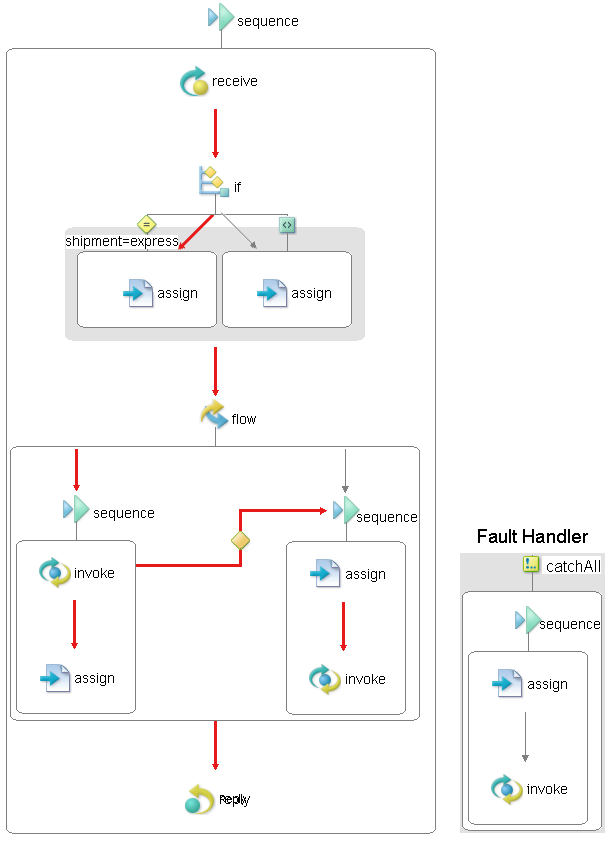
\includegraphics[width=0.6\textwidth]{bilder/Beispiel.png}
		\caption{Beispielprozess}
	\label{fig:Bespielprozess}
\end{figure}

Abh�ngig vom Liefertyp (\textit{express} oder \textit{normal}) werden die Bestellungsdaten unterschiedlich verarbeitet. Wenn der Kunde einen besonderen Status (VIP) hat, was mit dem \textit{Customer Identification}-Service festgestellt wird, dann wir der Kunde und sein Handelsvertreter �ber die Bestellung benachrichtigt.
Das wird mit Hilfe des Synchronisationslinks \textit{link\_1} modelliert, der eine explizite \textit{transition condition} aufweist: \textit{customerType='VIP'}.
F�r den Fehlerfall ist ein einfacher Fault Handler implementiert.

Der Prozess bekommt in einem Testfall eine Bestellung eines \textit{VIP}-Kunden mit folgenden Daten:
\begin{verbatim}
<order>
    <shipment>express</shipment>
    <customerId>12345</customerId>
    <productId>46298</productId>
</order>
\end{verbatim}

Es ist nur wichtig zu wissen, dass der Kunde den VIP-Status hat. Bei der Bearbeitung der Daten wird der mit roten Pfeilen markierte Pfad durchlaufen.
Mit der Erweiterung des BPELUnit-Frameworks kann die Testabdeckung ermittelt werden. Der Befehlszeilen-Client liefert die Testabdeckung im XML-Format:
\begin{verbatim}
<testingCoverage xmlns="http://www.bpelunit.org/schema/coverageResult">
  <FileStatistics filename="bpel/prozess.bpel">
    <statistic name="ActivityCoverage" totalItems="10" testedItems="7" />
    <statistic name="ActivityCoverage: assign" totalItems="5" 
                                                          testedItems="3" />
    <statistic name="ActivityCoverage: invoke" totalItems="3" 
                                                          testedItems="2" />
    <statistic name="ActivityCoverage: receive" totalItems="1" 
                                                          testedItems="1" />
    <statistic name="ActivityCoverage: reply" totalItems="1" 
                                                          testedItems="1" />
    <statistic name="BranchCoverage" totalItems="10" testedItems="8" />
    <statistic name="CompensationHandlerCoverage" totalItems="0" 
                                                          testedItems="0" />
    <statistic name="FaultHandlerCoverage" totalItems="1" testedItems="0" />
    <statistic name="LinkCoverage" totalItems="2" testedItems="1" />
    <statistic name="LinkCoverage: negativLinks" totalItems="1" 
                                                          testedItems="0" />
    <statistic name="LinkCoverage: positivLinks" totalItems="1" 
                                                          testedItems="1" />
  </FileStatistics>
</testingCoverage>
\end{verbatim}


Obwohl es sich um einen sehr einfachen BPEL-Prozess handelt, deckt ein Testfall   bereits 70\% der Basisaktivit�ten und 80\% der Zweige ab. Es wird allerding nur 50\% der Linkabdeckung erreicht und der Fault Handler wird gar nicht getestet. Der Tester kann diese Ergebnisse nutzen, um neue Testf�lle zu definieren und fehlende Bereiche abzudecken.